\documentclass[11pt]{article}
\usepackage[T1]{fontenc}
\usepackage[utf8]{inputenc}
\usepackage{lmodern}
\usepackage[letterpaper,margin=1in]{geometry}
\usepackage{amsmath,amssymb,amsthm,mathtools}
\usepackage{booktabs,longtable,tabularx,array,enumitem,microtype}
\usepackage{xcolor}
\usepackage{tikz}
\usetikzlibrary{arrows.meta,positioning,fit}
\usepackage[hidelinks]{hyperref}
\hypersetup{
  pdftitle={When Does a Physical Property Survive Representation Change?},
  pdfauthor={Anonymous author},
  pdfsubject={Uniform recovery, spectral rigidity, and the Yang--Mills representation chain}
}

% Central notation for Paper 03.
\newcommand{\Rep}{\mathfrak R}
\newcommand{\Aphys}{\mathcal A_{\mathrm{phys}}}
\newcommand{\Cert}{\mathsf C}
\newcommand{\Exact}{\mathsf E}
\newcommand{\Forgot}{\mathsf F}
\newcommand{\Recover}{\mathsf R}
\newcommand{\Uniform}{\mathsf U}
\newcommand{\Obs}{\mathcal O}
\newcommand{\Hilb}{\mathcal H}
\newcommand{\vac}{\Omega}
\newcommand{\spec}{\operatorname{spec}}
\newcommand{\supp}{\operatorname{supp}}
\newcommand{\e}{\mathrm e}
\newcommand{\id}{\mathrm{id}}


\newtheorem{theorem}{Theorem}[section]
\newtheorem{proposition}[theorem]{Proposition}
\newtheorem{lemma}[theorem]{Lemma}
\newtheorem{corollary}[theorem]{Corollary}
\theoremstyle{definition}
\newtheorem{definition}[theorem]{Definition}
\newtheorem{example}[theorem]{Example}
\newtheorem{counterexample}[theorem]{Counterexample}
\newtheorem{remark}[theorem]{Remark}

\title{When Does a Physical Property Survive Representation Change? Uniform Recovery, Spectral Rigidity, and the Yang--Mills Chain}
\author{Anonymous author}
\date{}

\begin{document}
\maketitle
\begin{abstract}
Physical properties are often generated, calculated, and interpreted in
different representations of a theory.  It does not follow that a property
made manifest in one description has been established for the physical
theory.  We develop a proof-bearing calculus for representation change in
which a morphism records, separately, exact preservation, quantitative
approximation, loss from the target variables, theorem-backed recovery, and
the index domain on which these claims are uniform.  The formal core is a
uniform recovery-to-spectrum theorem.  For positive semigroups, convergence
of Euclidean quadratic forms on a dense centered observable core, together
with one index-independent exponential rate, excludes target spectrum below
that rate.  Exact countermodels show that the conclusion fails as a physical
gap inference when the core is incomplete, finite-index rates collapse, or
cutoff and volume limits are interchanged without uniform recovery.  We use
four obstructions in lattice gauge reasoning to demonstrate that quantifier
domains, boundary charge, adaptive history, and partition-function
normalization are distinct forms of representational loss requiring different
repairs.  A complete Yang--Mills representation chain then identifies the
open interfaces between regulated local control, continuum Schwinger data,
Osterwalder--Schrader reconstruction, and a Hamiltonian mass gap.  The result
is a formal methodology for cross-representation warrant, compatible with
several realist and empiricist ontologies; it supplies no new construction of
four-dimensional continuum Yang--Mills theory.
\end{abstract}

\tableofcontents

\section{The fragmentation problem}
\label{sec:introduction}

A difficult result in mathematical physics is rarely proved in the variables
in which it receives its final physical interpretation.  Gauge potentials
make local dynamics tractable but contain redundancy.  Gauge-invariant
observables represent physical quantities more directly but can obscure local
coordinates.  A lattice regulator replaces an infinite-dimensional field
problem by finite group variables while breaking continuous spacetime
structure.  Renormalization reorganizes those variables by scale.  Euclidean
correlation functions expose positivity and probabilistic control.  A
Hamiltonian representation finally turns long-time behavior into a spectral
statement.  Each description is useful because it displays some structure
and suppresses other structure.

This plurality creates a logical problem that is sharper than the familiar
observation that models are partial.  Suppose an estimate is proved after
gauge fixing, coarse graining, finite-volume restriction, or passage to a
Euclidean measure.  Which part of the estimate belongs to the physical theory,
and which part belongs to the chosen representation?  What must be shown
before a local contraction becomes a statement about continuum
correlations, or before exponential Euclidean decay becomes a Hamiltonian
mass gap?  A general appeal to equivalence is inadequate because the relevant
maps are often irreversible, approximate, indexed by singular limits, or
equivalent only on a restricted algebra of observables.

The philosophy of physics already provides indispensable pieces of the
answer.  Structural realism asks which structure merits realist commitment
through theory change \cite{Worrall1989,VanFraassen2006,Roberts2011}.
Work on gauge symmetry distinguishes reduction, sophistication, and surplus
structure, including the role that unreduced variables can play in
representing local fields \cite{Belot2003,Dewar2019,NguyenTehWells2020}.
Accounts of theoretical equivalence and duality separate formal isomorphism
from interpretation \cite{Coffey2014,Lupher2018,DeHaroButterfield2018}.
Functorial quantum field theory makes covariance and inter-model maps
mathematically precise \cite{BrunettiFredenhagenVerch2003,Fewster2015}.
Renormalization-group and effective-field-theory scholarship shows that scale
transformation has several technically and epistemically different forms
\cite{WilsonKogut1974,Butterfield2011,Rivat2021,KoberinskiFraser2023}.
Recent work on perspicuous representation further argues that physical
formulations are not selected by convention alone \cite{North2026}.

These approaches mostly ask what theories, models, structures, or
perspectives are, when descriptions are equivalent, or why one formulation
is more revealing.  The present question is narrower and proof-directed:

\begin{quote}
When does a property proved in one representation survive a chain of
nonexact transformations and count as established in a limiting physical
representation?
\end{quote}

We answer by associating each transformation with a \emph{certificate
profile}.  A profile is not a global label such as ``faithful.''  It records
which property channels are exact, which have observable-dependent error
moduli, which are unavailable in the target variables, which are recovered by
a separate theorem, and over which cutoff, volume, scale, distance, and
observable quantifiers the certificate is uniform.  We call the resulting
analysis \emph{proof-bearing representational dynamics}.  The qualifier is
essential: ``representational dynamics'' already names temporal changes of
internal representations in cognitive science and machine learning.  Here it
means transformations among scientific descriptions together with proof
objects for claim transport.

The paper makes four contributions.  First, it defines a typed representation
package containing a redundancy groupoid, a physical observable algebra,
positive states, dynamics or correlations, scale/limit data, and certified
properties.  Its morphisms distinguish exact preservation, approximation,
forgetting, and recovery.  Their error moduli compose by typed pullback rather
than by collapsing every property into one number.

Second, we prove a recovery-to-spectrum theorem.  Consider positive
semigroups generated by $H_i\geq0$ and a target $H\geq0$.  If recovered
quadratic forms converge on a centered core that is dense in the target
vacuum complement, and if every regulated form obeys one exponential rate
$m>0$ uniformly in the index, then
\[
  \spec(H)\cap(0,m)=\varnothing.
\]
The mechanism is positivity of the spectral measure, followed by density of
the core.  The theorem is elementary as spectral analysis; its role is to
make four prerequisites of a physical inference inseparable: positivity,
correlation recovery, observable completeness, and uniform physical scale.
It therefore exceeds a Boolean certificate conjunction or a scalar
error-summing rule.

Third, three exact countermodels establish the independence of those
prerequisites.  A nonseparating core can miss a lower-energy sector.  A
sequence of finite systems can have a positive gap at every index while the
gaps converge to zero.  A recovery defect can vanish at each fixed volume but
remain one after the infinite-volume limit.  These are not pathological
decorations; they reproduce the logical forms of common shortcuts in
constructive field theory.

Fourth, the Yang--Mills existence and mass-gap problem provides a sustained
case rather than a motivational slogan.  We track locality, gauge invariance,
positivity, scale dependence, observable completeness, and spectrum from
lattice link variables through gauge quotient and block transformation to
continuum Schwinger data, Osterwalder--Schrader (OS) reconstruction, and a
Hamiltonian.  Four concrete failures of proposed lattice estimates are
classified as losses of quantifier domain, boundary state, adaptive history,
and normalization.  The classification is methodologically effective because
each loss selects a different mathematical repair.

The official problem asks for a nontrivial quantum Yang--Mills theory on
$\mathbb R^4$ and a positive Hamiltonian mass gap
\cite{JaffeWitten2000}.  Nothing here constructs that continuum theory or
proves the uniform infrared estimate needed to apply the central theorem.
The Yang--Mills contribution is a precise interface theorem and a conservative
frontier diagnosis.  The formal result is a conditional representation-
transfer theorem; the physical premises remain open.

Section~\ref{sec:levels} separates ontology, semantics, epistemology, and
proof methodology.  Sections~\ref{sec:calculus}--\ref{sec:countermodels}
develop the calculus, theorem, and countermodels.  Sections~\ref{sec:ymchain}
and~\ref{sec:failures} analyze Yang--Mills.  Sections~\ref{sec:ontology}
and~\ref{sec:related} locate the framework philosophically, after which
Sections~\ref{sec:objections} and~\ref{sec:discussion} address objections and
research consequences.  Appendices contain complete definitions, proofs,
the property-transport table, and exact finite reproducibility artifacts.

\section{Four levels that must not be conflated}
\label{sec:levels}

The word ``representation'' can connect questions about reality, meaning,
warrant, and proof.  Moving among these levels without notice makes an
apparently deep thesis either trivial or overstated.  We therefore separate
four claims.

\subsection{Ontology}

An ontological claim concerns what exists or is fundamental: objects,
relations, events, fields, algebraic structures, or something else.  The
formalism developed below does not select among these options.  It supports a
more modest thought: when one physical theory is realized through several
descriptions, the content for which cross-description recovery can be proved
is a particularly robust candidate for objective commitment.  That is
compatible with ontic or epistemic structural realism, entity realism,
constructive empiricism, and pragmatism.  It does not imply that the universe
literally is a diagram or that relations exist without relata.

\subsection{Semantics}

A semantic claim specifies what mathematical items represent and under which
interpretation.  A gauge potential, an orbit, a Wilson loop, a probability
measure, a blocked action, a Schwinger functional, and a spectral projection
do not represent the same type of thing.  Their physical content depends on
an observable algebra, states that assign expectation values, a redundancy
relation, and an interpretation of dynamics and units.  Two structures can
be isomorphic while receiving different interpretations; conversely,
nonisomorphic models can agree on a restricted empirical domain
\cite{Coffey2014,DeHaroButterfield2018}.  The calculus consequently types both
formal maps and the claims transported by them.

\subsection{Epistemology}

The epistemic issue is when a result in one description warrants a result in
another.  The answer is property-relative.  A gauge quotient can be exact for
invariant expectation values while losing manifest local sections.  A coarse
graining can approximate long-distance observables while erasing a boundary
state needed for conditional estimates.  A Euclidean functional can encode a
Hamiltonian spectrum only when positivity and reconstruction hypotheses hold.
There is no contradiction in assigning different fidelity verdicts to the
same arrow, because the predicates have different bearers and inferential
roles.

\subsection{Proof methodology}

The methodological claim is operational.  A proof that crosses a
representation interface must record:
\begin{enumerate}[label=(\roman*),itemsep=2pt]
  \item the source and target objects;
  \item the observable or state map and its domain;
  \item the target property and all of its prerequisites;
  \item exact equations or approximation moduli;
  \item structures unavailable in the target variables;
  \item separate recovery theorems; and
  \item the order and uniformity of all limiting quantifiers.
\end{enumerate}
This is the level on which the paper's formal results operate.  The utility of
the calculus does not wait on settlement of the ontology.

\subsection{A dispensable use of information}

The phrase ``physical information'' is often asked to perform work belonging
to all four levels.  We use it only as shorthand for distinctions among
states that are recoverable by a declared family of physical observables.  Its
bearer is a state or correlation functional; its equivalence relation is
agreement on the physical algebra; its accessibility is the state--observable
pairing; and its dynamics is a typed action on those pairings.  Gauge change,
physical time evolution, RG transformation, and OS reconstruction are thus
different operations.  If bearer, equivalence relation, and inferential role
are absent, the word ``information'' can be deleted without changing the
framework.  This prevents an informational slogan from substituting for a
physical ontology.

\section{A proof-bearing calculus of representation change}
\label{sec:calculus}

The calculus is intentionally small.  It does not attempt to encode every
feature of a physical theory.  It records the objects needed to decide whether
a particular claim can cross a particular interface.

\subsection{Representation packages}

\begin{definition}[Representation package]
\label{def:package}
A \emph{representation package} is a tuple
\[
 \Rep=(\mathcal K,\mathcal G,\Aphys,\mathcal S,\mathcal T,
       \mathcal L,\mathcal Q)
\]
with the following typed components.
\begin{enumerate}[label=(\roman*),itemsep=2pt]
 \item $\mathcal G\rightrightarrows\mathcal K$ is a groupoid of
 kinematical presentations and redundancies.
 \item $\Aphys$ is a unital $*$-algebra of physical observables, equipped
 with seminorms $p_\alpha$ and an interpretation of support.
 \item $\mathcal S\subset\Aphys^{*}$ is a specified class of normalized
 positive states.
 \item $\mathcal T$ is physical time evolution, a Euclidean correlation
 family, or another explicitly typed dynamics; these alternatives are not
 identified.
 \item $\mathcal L=(I,\preceq,\lambda,\mathfrak C)$ records the directed
 index set, physical scales and units, admissible limiting paths, and
 convergence topologies.
 \item $\mathcal Q$ is a family of property predicates, each with a bearer,
 domain, units, and quantifier prefix.
\end{enumerate}
The algebra $\Aphys$ is invariant under $\mathcal G$, or is supplied with a
descent theorem from a covariant algebra.
\end{definition}

The groupoid accommodates the fact that a gauge transformation relates
presentations rather than physical histories.  The distinction between
$\mathcal T$ and $\mathcal L$ prevents physical time from being identified
with an RG parameter.  The property set $\mathcal Q$ is not a list of words:
``locality,'' for example, must specify a net or support rule, while ``gap''
must specify a generator, a vacuum sector, and physical energy units.
Appendix~\ref{app:typed} gives the full typing and identity conditions.

\begin{example}[Finite semigroup package]
Let $\mathcal K=\mathbb C^{d}$, let the redundancy groupoid be trivial, let
$\Aphys=M_d(\mathbb C)$, and let $\mathcal S$ be density matrices.  A positive
self-adjoint $H$ defines $\mathcal T_t(A)=\e^{-tH}A\e^{-tH}$ for Euclidean
quadratic forms.  The limit data may be a sequence of inclusions into a
separable Hilbert space.  Spectral support, core completeness, and semigroup
decay are well-typed property predicates.
\end{example}

\begin{example}[Regulated lattice gauge package]
For a finite lattice, $\mathcal K=G^{E}$, the vertex gauge group acts as a
groupoid of link presentations, and $\Aphys$ is a chosen algebra of invariant
functions.  A positive lattice measure defines states and Euclidean
correlations.  The limit data include lattice spacing, physical volume,
bare/renormalized parameters, and observable renormalization.  Gauge
invariance is exact at finite cutoff, while continuum covariance, physical
observable completeness, and a Hamiltonian gap are limit or reconstruction
predicates.  This instantiates every component without treating the regulator
as the continuum theory.
\end{example}

\subsection{Certificate-profiled morphisms}

Let $F:\Rep_0\to\Rep_1$ contain a pullback
$F^*: \mathcal D_1\to\Aphys^{(0)}$ on a declared target-observable domain and,
when defined, a state pushforward $F_*:\mathcal S_0\to\mathcal S_1$.  Exact
duality would require
\[
 \langle F_*\omega,A\rangle
   =\langle\omega,F^*A\rangle.
\]
Approximate, limiting, and coarse-graining maps instead carry a family
$\varepsilon_F(A;i)$ satisfying
\begin{equation}
\label{eq:fidelity}
 \left|\langle F_*\omega,A\rangle-
        \langle\omega,F^*A\rangle\right|
 \leq \varepsilon_F(A;i)
\end{equation}
for the stated states, observables, and indices.

\begin{definition}[Certificate profile]
\label{def:profile}
The profile of $F$ is
\[
 \Cert(F)=(\Exact_F,\varepsilon_F,\Forgot_F,\Recover_F,\Uniform_F).
\]
$\Exact_F$ contains exact property channels.  $\varepsilon_F$ is a
heterogeneous family of observable-dependent moduli.  $\Forgot_F$ lists
structures not available in the target variables.  $\Recover_F$ contains
theorems or partial sections that recover specified claims despite such loss.
$\Uniform_F$ records the full index domain and order of quantifiers on which
each entry holds.
\end{definition}

Forgetting is therefore not the negation of physical existence.  It says that
the target representation does not by itself carry a datum required by the
inference.  Recovery is not a declaration that the datum ``must still be
there.''  It names a map or theorem, its domain, and a modulus.  Exact
inverses, reconstruction on an observable core, asymptotic recovery, and
external reconstruction theorems are consequently different entries.

Figure~\ref{fig:profile} displays the logical form.  The arrow can preserve
some channels and erase others; a recovery theorem is a second arrow, not an
optimistic interpretation of the first.

\begin{figure}[t]
\centering
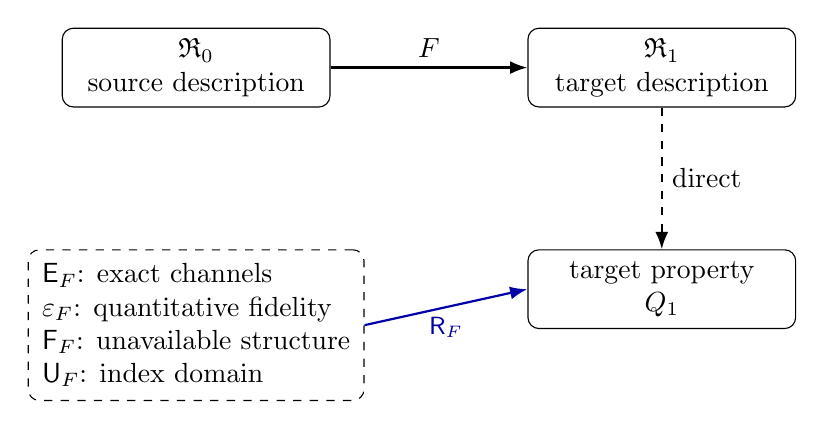
\begin{tikzpicture}[
  box/.style={draw,rounded corners,align=center,minimum width=34mm,minimum height=10mm},
  cert/.style={draw,dashed,rounded corners,align=left,inner sep=5pt},
  arr/.style={-{Latex[length=2.2mm]},thick},
  node distance=18mm and 25mm]
\node[box] (r0) {$\Rep_0$\\source description};
\node[box,right=of r0] (r1) {$\Rep_1$\\target description};
\draw[arr] (r0) -- node[above] {$F$} (r1);
\node[cert,below=of r0] (c)
 {$\Exact_F$: exact channels\\
  $\varepsilon_F$: quantitative fidelity\\
  $\Forgot_F$: unavailable structure\\
  $\Uniform_F$: index domain};
\node[box,below=of r1] (p) {target property\\$Q_1$};
\draw[arr,dashed] (r1) -- node[right] {direct} (p);
\draw[arr,blue!65!black] (c.east) --
 node[below,align=center,font=\small] {$\Recover_F$} (p.west);
\end{tikzpicture}
\caption{A property-relative representation morphism.  Recovery is a
separate theorem-backed route from the source data and certificate profile to
the target claim.}
\label{fig:profile}
\end{figure}

\subsection{Composition without scalarization}

Suppose $F:\Rep_0\to\Rep_1$ and $G:\Rep_1\to\Rep_2$.  For a target
observable $B$, inserting the intermediate expectation gives
\begin{equation}
\label{eq:composition}
 \varepsilon_{G\circ F}(B;i)
 \leq \varepsilon_G(B;i)+\varepsilon_F(G^*B;i).
\end{equation}
If the pullback of $G$ obeys
$p_1(G^*B)\leq L_G(B)p_2(B)$ and the first error is controlled by $p_1$,
then
\[
 \varepsilon_{G\circ F}(B;i)
 \leq \varepsilon_G(B;i)+L_G(B)\varepsilon_F(B;i).
\]
Locality range, positivity, gauge descent, and spectral fidelity are not
folded into this scalar expression.  Each has its own composition rule and
failure mode.

\begin{proposition}[Typed profile composition]
\label{prop:composition}
On composable observable domains, expectation moduli compose by
Equation~\eqref{eq:composition}; exact channels compose by conjunction;
uniformity domains compose by intersection with the pulled-back quantifier
order; and a forgotten prerequisite can appear in the composite conclusion
only through an explicit recovery theorem.  For three composable morphisms,
the expectation modulus is associative:
\[
 \varepsilon_H+L_H\varepsilon_G+L_HL_G\varepsilon_F,
\]
independently of bracketing.
\end{proposition}

The proof is in Appendix~\ref{app:composition}.  This proposition is still
bookkeeping.  Its importance is negative and architectural: it prevents one
successful channel from licensing another.  The substantive result comes
when a recovery theorem turns a family of Euclidean bounds into a spectral
property.

\subsection{How much category theory is claimed?}

Exact representation equivalences, with total observable maps and identities,
form an ordinary category.  Approximate arrows with seminorm-valued profiles
can be organized in enriched or ordered structures, and institution-style
semantics provides useful analogies for invariance under change of notation
\cite{GoguenBurstall1992}.  We do not claim that every coarse graining,
limiting correspondence, or partial reconstruction belongs to one completed
category.  In the present paper, ``morphism'' means a typed composable arrow
on the stated domain.  Categorical vocabulary is retained only where identity
and associativity have been proved.

\section{Uniform recovery and spectral rigidity}
\label{sec:recovery}

The central case concerns a property whose natural bearer changes.  In a
Euclidean representation one proves decay of positive correlation forms.  In
a Hamiltonian representation the desired statement is absence of spectral
weight at low positive energy.  The bridge uses the OS reconstruction
paradigm \cite{OsterwalderSchrader1973,OsterwalderSchrader1975}, but the
abstract argument needs only positive semigroups and a dense recovered core.

\begin{definition}[Indexed semigroup recovery system]
\label{def:recovery}
Let $(I,\preceq)$ be directed.  For each $i\in I$, let $H_i\geq0$ be
self-adjoint on $\Hilb_i$.  Let $H\geq0$ be self-adjoint on $\Hilb$, with
distinguished unit vacuum $\vac$ and $\ker H=\mathbb C\vac$.  An indexed
semigroup recovery system consists of a linear subspace
$\mathcal D\subset\vac^\perp$ and eventually defined vectors
$J_i x\in\Hilb_i$ for $x\in\mathcal D$ such that, for every $t\geq0$,
\begin{equation}
\label{eq:semigroup-recovery}
 \langle J_i x,\e^{-tH_i}J_i x\rangle
 \longrightarrow
 \langle x,\e^{-tH}x\rangle.
\end{equation}
The system is \emph{complete} when $\mathcal D$ is dense in $\vac^\perp$.
It has \emph{uniform rigidity at rate $m$} when one $m>0$ exists such that,
for every $x\in\mathcal D$, a finite $M_x$ and index $i_x$ satisfy
\begin{equation}
\label{eq:uniform-rigidity}
 \langle J_i x,\e^{-tH_i}J_i x\rangle
 \leq M_x\e^{-mt}
 \quad (i\succeq i_x,\ t\geq0).
\end{equation}
\end{definition}

The common rate $m$ is uniform in the regulator index and is expressed in the
target physical time variable.  The prefactor may depend on the observable
vector, because spectral exclusion is established vector by vector before
density is used.  Equation~\eqref{eq:semigroup-recovery} may be obtained from
an explicit error modulus $\rho_i(x,t)$ that vanishes for every fixed $x,t$.

\begin{theorem}[Uniform recovery-to-spectrum]
\label{thm:recovery-spectrum}
Every complete indexed semigroup recovery system with uniform rigidity at
rate $m>0$ satisfies
\[
  \spec(H)\cap(0,m)=\varnothing.
\]
Equivalently, the target Hamiltonian has gap at least $m$ above its unique
vacuum.
\end{theorem}

\paragraph{Proof mechanism.}
For $x\in\mathcal D$, positivity and the spectral theorem give a positive
measure $\mu_x$ with
\[
 \langle x,\e^{-tH}x\rangle
   =\int_{[0,\infty)}\e^{-t\lambda}\,d\mu_x(\lambda).
\]
Taking the index limit in Equation~\eqref{eq:uniform-rigidity} gives an
$\e^{-mt}$ upper bound.  Any positive $\mu_x$-mass below $m$ would decay more
slowly and contradict that bound at large $t$.  Hence the spectral projection
$E_H((0,m))$ annihilates every $x\in\mathcal D$.  Density of $\mathcal D$ in
$\vac^\perp$ and boundedness of the projection imply
$E_H((0,m))=0$.  Appendix~\ref{app:spectral} gives the full proof and isolates
where positivity, centering, and density enter.

The theorem does not merely add representation errors.  It changes the type
of the property: a family of inequalities for recovered Euclidean quadratic
forms becomes a statement about the support of a target projection-valued
measure.  Positivity makes that transition possible; completeness makes it
global rather than sectorial; and uniformity prevents low-energy states from
escaping along the limiting index.

\begin{corollary}[OS-positive correlation-to-gap interface]
\label{cor:os}
Suppose a limiting Euclidean functional satisfies the hypotheses required for
OS reconstruction and yields $(\Hilb,\vac,H)$.  Suppose further that centered
vectors created by a gauge-invariant observable core are dense in
$\vac^\perp$, their regulated two-point forms converge to the reconstructed
semigroup forms, and Equation~\eqref{eq:uniform-rigidity} holds in physical
Euclidean time.  Then the reconstructed Hamiltonian has gap at least $m$.
\end{corollary}

This corollary is an interface theorem.  It does not prove OS positivity,
observable density, convergence of renormalized correlations, or the uniform
decay estimate for any particular interacting four-dimensional theory.

\subsection{A successful transport chain}

The elementary sequence
\[
 H_n=\operatorname{diag}(0,1,2,\ldots,n)
\]
embeds into $\mathbb C\vac\oplus\ell^2(\mathbb N)$ with target
$H\,e_k=k e_k$.  Every finite-support centered vector is recovered exactly
for all sufficiently large $n$; every regulated quadratic form decays at
least as $\e^{-t}$; finite-support vectors are dense; and the target gap is
one.  This example is simple, but it shows the complete logical chain:
carrier recovery, dynamical fidelity, a uniform rate, dense-core recovery,
and spectral interpretation.  The exact supplement checks its finite
truncations.  The counterexamples in the next section remove one certificate
at a time.

\section{Why pointwise recovery is insufficient}
\label{sec:countermodels}

The central hypotheses are logically independent.  Three exact examples
display the corresponding false positives.

\subsection{A hidden low-energy sector}

\begin{counterexample}[Incomplete observable core]
\label{ex:hidden}
Let
\[
 H=\operatorname{diag}(0,1,\tfrac12)
\]
on $\mathbb C^3$, with the first vector as vacuum.  If the declared observable
core creates only the energy-one vector, every tested centered correlation is
exactly $\e^{-t}$ times its norm.  Nevertheless the physical gap is
$1/2$.  The tested core is not dense in the vacuum complement.
\end{counterexample}

This is the finite form of a sectorial result.  A collection of local or
symmetry-restricted observables may display a rate that says nothing about an
orthogonal physical sector.  The repair is not a smaller error bar; it is a
density or state-separation theorem.

\subsection{Positive finite gaps that collapse}

\begin{counterexample}[Escaping low-energy states]
\label{ex:collapse}
For $n\geq1$, let
\[
 H_n=\operatorname{diag}(0,1,\tfrac12,\ldots,\tfrac1n)
\]
and include its Hilbert space into
$\mathbb C\vac\oplus\ell^2(\mathbb N)$.  The direct-limit generator satisfies
$H e_k=k^{-1}e_k$.  Every $H_n$ has a positive gap $1/n$, and every fixed
finite-support vector and its semigroup correlation are eventually recovered
exactly.  Yet $H$ is gapless because its positive spectrum accumulates at
zero.
\end{counterexample}

Thus ``there exists $m_n>0$ for every regulator'' does not approach the
quantifier ``there exists $m>0$ for every sufficiently refined regulator.''
If the lattice spacing is present, the rate must additionally be converted to
physical units before the infimum is taken.

\subsection{A noncommuting recovery defect}

\begin{counterexample}[Cutoff versus volume]
\label{ex:limits}
For positive integers $n,L$, define
\[
 d(n,L)=\mathbf 1_{\{L>n\}}.
\]
At every fixed volume, $d(n,L)\to0$ as $n\to\infty$.  At every fixed cutoff
index, $d(n,L)\to1$ as $L\to\infty$.  Consequently
\[
 \lim_{L\to\infty}\lim_{n\to\infty}d(n,L)=0,
 \qquad
 \lim_{n\to\infty}\lim_{L\to\infty}d(n,L)=1,
\]
and $\sup_L d(n,L)=1$ for every $n$.
\end{counterexample}

The example turns ``uniform'' into a visible quantifier.  A proof at each
fixed volume can be correct and still fail to define an infinite-volume
property.  Appendix~\ref{app:countermodels} gives the direct-limit operator
details and the finite exact certificate.

\subsection{What the countermodels establish}

The three failures cannot be represented by a single larger scalar error.
The hidden-sector example lacks a completeness theorem.  The collapsing-gap
example lacks a uniform physical rate.  The defect array lacks control of the
order of limits.  A proof-bearing profile distinguishes these types so that a
successful estimate in one channel cannot conceal a missing theorem in
another.

\section{Yang--Mills as a full-chain test}
\label{sec:ymchain}

The Yang--Mills problem is unusually revealing because the structures needed
for the conclusion are naturally distributed across representations.  The
official target combines existence of a nontrivial continuum quantum field
theory with a positive Hamiltonian mass gap \cite{JaffeWitten2000}.  A finite
lattice construction makes neither conjunct automatic.

\subsection{The representation chain}

Fix a compact simple gauge group $G$.  A constructive route may begin with
lattice link variables at spacing $a$ and physical volume $L$, pass to
gauge-orbit data, integrate fluctuations into block variables, take volume
and cutoff limits of renormalized gauge-invariant observables, reconstruct a
Hilbert-space theory, and finally interpret Euclidean decay spectrally:

\begin{figure}[t]
\centering
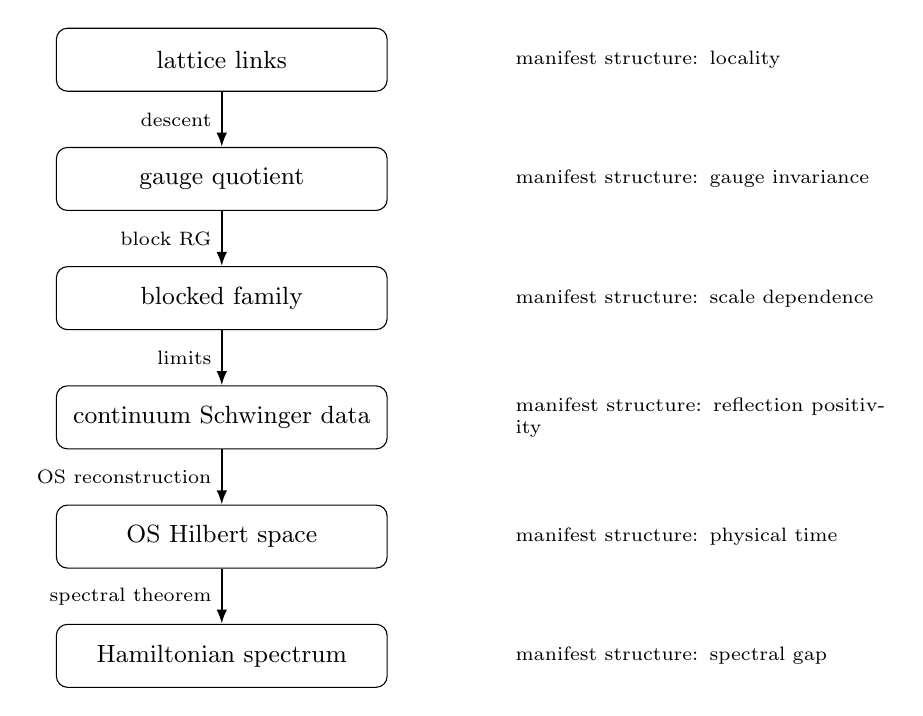
\begin{tikzpicture}[
  node distance=7mm,
  box/.style={draw,rounded corners,align=center,minimum width=42mm,
    minimum height=8mm,font=\small},
  arr/.style={-{Latex[length=1.8mm]},thick},
  lab/.style={font=\scriptsize,align=left},
  exposed/.style={font=\scriptsize,align=left,text width=47mm}]
\node[box] (lat) {lattice links};
\node[box,below=of lat] (quo) {gauge quotient};
\node[box,below=of quo] (rg) {blocked family};
\node[box,below=of rg] (sch) {continuum Schwinger data};
\node[box,below=of sch] (os) {OS Hilbert space};
\node[box,below=of os] (sp) {Hamiltonian spectrum};
\draw[arr] (lat) -- node[left,lab] {descent} (quo);
\draw[arr] (quo) -- node[left,lab] {block RG} (rg);
\draw[arr] (rg) -- node[left,lab] {limits} (sch);
\draw[arr] (sch) -- node[left,lab] {OS reconstruction} (os);
\draw[arr] (os) -- node[left,lab] {spectral theorem} (sp);
\node[exposed,right=15mm of lat] {manifest structure: locality};
\node[exposed,right=15mm of quo] {manifest structure: gauge invariance};
\node[exposed,right=15mm of rg] {manifest structure: scale dependence};
\node[exposed,right=15mm of sch] {manifest structure: reflection positivity};
\node[exposed,right=15mm of os] {manifest structure: physical time};
\node[exposed,right=15mm of sp] {manifest structure: spectral gap};
\end{tikzpicture}
\caption{The Yang--Mills representation chain.  The labels to the right of the nodes
name structures naturally exposed there, not properties absent everywhere
else.  Every arrow has separate preservation and recovery obligations.}
\label{fig:ymchain}
\end{figure}

The chain is not a chronology and no node is globally superior.  It is an
interface graph.  The main obligations are as follows.

\paragraph{Gauge descent.}
The quotient must preserve the physical observable algebra and measure while
accounting for orbit singularities, residual gauge transformations, and
topological sectors.  A local gauge chart can be exact on its domain without
covering the full measure.  Conversely, unreduced variables can carry useful
local structure even when they are redundant; this is consonant with the
locality analysis of surplus gauge structure
\cite{NguyenTehWells2020}.

\paragraph{Scale transformation.}
An RG step changes variables and often the form or range of the action.  Its
physical meaning depends on the specific RG construction; coarse graining is
not synonymous with every use of the renormalization group
\cite{KoberinskiFraser2023}.  For a constructive proof, the map must retain a
state sufficient to reconstruct the required observables and must control
positivity, locality range, large fields, boundary conditions, and topology.

\paragraph{Infinite volume and continuum.}
One needs normalized gauge-invariant observables whose correlation
functionals converge in a declared distributional topology, together with
reflection positivity, Euclidean covariance, clustering or another vacuum
selection condition, nontriviality, and regulator independence.  Constants
must be uniform in $L$ before $L\to\infty$ and stable in physical units as
$a\downarrow0$.  A subsequential symmetric limit is not automatically the
intended pure Yang--Mills theory.

\paragraph{Reconstruction and spectral interpretation.}
The OS axioms provide a theorem-backed route from suitable Euclidean data to
a Hilbert space and positive Hamiltonian
\cite{OsterwalderSchrader1973,OsterwalderSchrader1975}.  To infer a global gap
from decay, the centered gauge-invariant core used in the estimate must be
dense in the reconstructed vacuum complement.  Theorem
\ref{thm:recovery-spectrum} then performs only the final inference; it cannot
supply the Euclidean estimate or the continuum object.

\subsection{Property visibility}

The decisive properties do not line up in one column.  Lattice variables make
local action and exact finite gauge covariance explicit.  The quotient makes
physical invariance explicit but can hide local sections.  RG variables make
scale dependence explicit but can hide microscopic locality and normalized
boundary data.  Schwinger functions make Euclidean correlation structure
explicit, while a Hamiltonian makes spectrum explicit.  Reflection
positivity is an action- and interface-specific certificate, not an automatic
benefit of Euclidean notation.  Appendix~\ref{app:ymtable} supplies the full
visibility and obligation matrix.

\subsection{The exact first open physical implication}

The chain isolates a frontier before OS reconstruction.  One needs a
gauge-invariant observable core $\mathcal D_{a,L}$ and constants in physical
units such that, schematically,
\begin{equation}
\label{eq:ym-rigidity}
 \left|\langle A\,\tau_t(B)\rangle_{a,L,c}\right|
 \leq C_{A,B}\e^{-mt}+r_{a,L}(A,B,t),
\end{equation}
with $m>0$ and admissible prefactors uniform in volume and sufficiently small
cutoff, and with recovery errors converging in the topology used for the
Schwinger limit.  The statement must cover a core that becomes dense after
reconstruction.  It may be generated by RG contraction, a polymer expansion,
a transfer estimate, or another noncircular rigidity engine.  Assuming
all-distance exponential clustering as an input would merely assume the
needed property in a different representation.

No result in this paper proves Equation~\eqref{eq:ym-rigidity} for
four-dimensional weak-coupling pure Yang--Mills, nor does it prove the
continuum premises.  The contribution is the implication boundary: local or
finite spectral rigidity counts as a physical mass gap only after the
full-measure, uniform, continuum, positivity, completeness, and reconstruction
certificates close.

\section{Four forms of loss in lattice gauge reasoning}
\label{sec:failures}

The calculus earns methodological content only if it differentiates failures
that ordinary language treats alike.  We analyze four exact logical forms.
Each begins from a natural estimate and ends with a different repair.

\subsection{Loss of the admissible quantifier domain}

Let $p_t$ be a heat kernel on a compact connected group.  As $t\downarrow0$,
$p_t(g^{-1}\,\cdot)$ concentrates near $g$.  If $g\neq h$, choose disjoint
neighborhoods of the two points.  Concentration then implies
\begin{equation}
\label{eq:tv-translate}
 \left\|p_t(g^{-1}\,\cdot)-p_t(h^{-1}\,\cdot)\right\|_{\mathrm{TV}}
 \longrightarrow 1.
\end{equation}
A worst-translate influence coefficient therefore becomes maximally bad in
the small-time regime where the local measure is most concentrated.

The estimate is correct; its proposed interpretation is not.  Arbitrary
group translates need not correspond to neighboring conditionings inside the
same physically coherent small-field collar.  The representation has exposed
translation and concentration while suppressing the admissibility relation
among boundary states.  The repair is to type the supremum: compare only
conditionings connected by a certified good collar, and treat the complement
through a charged defect or polymer channel.  Replacing the total-variation
constant by a more optimistic local calculation would not repair the missing
quantifier domain.

\subsection{Loss of boundary charge}

Consider one $SU(2)$ link with six incident plaquette staples.  A center-valued
boundary can arrange five identity staples and one $-I$ staple.  For a
heat-kernel plaquette weight, the exact conditional density is proportional
to
\begin{equation}
\label{eq:frustrated-density}
 p_t(U)^5p_t(-U)\,dU.
\end{equation}
Write $\theta\in[0,\pi]$ for the class angle of $U$.  The small-time rate is,
up to the common heat-kernel normalization,
\[
 I(\theta)=5\theta^2+(\pi-\theta)^2.
\]
It is minimized at $\theta=\pi/6$.  The plaquette facing the negative staple
then has angle $5\pi/6$: the one-link conditional is not concentrated on a
configuration in which every adjacent plaquette is small.

The boundary pattern itself carries an action cost.  Conditioning on it and
then demanding a boundary-uniform one-link estimate erases that cost from the
probability accounting.  The repair is a retained boundary charge, a
multi-link integration, or a contour variable that assigns the frustration
to the correct state.  The failed statement was uniform over a state space
too small to remember why the hostile conditioning was rare.

\subsection{Loss of adaptive history}

Fixed intersection moments need not control sequential conditionals.  Let
$0<q<1$ and let Bernoulli variables satisfy
\[
 \mathbb P(X_1=X_2=1)=q^2,
 \qquad
 \mathbb P(X_1=X_2=0)=1-q^2.
\]
Then $\mathbb P(X_j=1)=q^2\leq q$ and
$\mathbb P(X_1=X_2=1)=q^2$, so the one- and two-site intersection bounds
match the familiar powers of $q$.  Nevertheless
\[
 \mathbb P(X_2=1\mid X_1=1)=1.
\]
The intersection data have forgotten which history was revealed before the
next choice.  Adaptive domination needs a filtration-indexed state or a
uniform conditional theorem.  More moments of the same untyped kind do not
automatically recover the history.

\subsection{Loss of normalization}

For a defect event $B$ under boundary state $y$, the exact probability is
\begin{equation}
\label{eq:partition-ratio}
 \mathbb P_y(B)=\frac{Z_B(y)}{Z(y)}.
\end{equation}
An action lower bound on configurations in $B$ controls a numerator.  It does
not control the ratio unless the denominator, or a suitable reference
free-energy difference, is bounded on the same state domain.  A hostile
boundary can suppress $Z(y)$ at the same exponential scale as $Z_B(y)$.
The representation by unnormalized action charge has forgotten entropy and
normalization.  Recovery requires a conditional partition-ratio theorem, not
only a stronger energetic inequality.

\subsection{Why the distinctions matter}

The four repairs enlarge different parts of the representation package:
admissible boundary relations, retained center/topological state, adaptive
filtration, and normalized free energy.  They cannot be ranked on a single
fidelity scale.  This is the practical content of certificate profiles.  A
failed proof becomes a typed diagnosis of which state or theorem is missing,
rather than a generic verdict that the approximation was too crude.

\section{What ontology, if any, follows?}
\label{sec:ontology}

The formal picture invites a metaphysical gloss.  Gauge fields may be called
coordinates on physical information; regulators temporary realizations;
particles spectral interpretations; renormalization a transformation of
descriptive scale; the continuum a coherence condition; and the mass gap an
invariant form of infrared rigidity.  These phrases are useful only after
their logical strength is reduced.

\subsection{Stable objects as recovered invariants}

One defensible thesis is that a physical object or property is stable to the
extent that its inferential role is recovered across a sufficiently rich
class of admissible representations.  ``Recovered'' is stronger than
numerical resemblance.  It means that state distinctions, observable values,
causal or dynamical relations, and relevant limits are transported by a
profile whose failures are known.  A particle, for example, is not a link
variable carried unchanged through RG.  It is a spectral interpretation in a
Hamiltonian representation, related to Euclidean correlations through a
reconstruction theorem.

This view can accommodate entities.  An object may be the stable bearer of a
family of recovered relations rather than something eliminated in favor of
relations.  It also accommodates representation-dependent manifestation: a
property can be real without being explicit in every coordinate system.

\subsection{Why this is not automatically structural realism}

Worrall's structural realism identifies continuity of structure as a possible
realist commitment through theory change \cite{Worrall1989}.  The present
calculus is sympathetic to selective commitment but does not identify one
privileged structure.  Certificate profiles presuppose typed objects,
observables, states, and maps.  Roberts's objection that structures themselves
have structure warns against an unmotivated hierarchy
\cite{Roberts2011}; van Fraassen's critique warns that bare structural claims
can be too weak to carry the desired realism \cite{VanFraassen2006}.
Property-relative recovery supplies modal and inferential detail, but it does
not prove that relations are ontologically prior to relata.

\subsection{Four compatible readings}

An ontic structural realist may treat the maximally coherent network of
recovered relations as fundamental.  An entity realist may treat cross-
representation intervention and recovery as evidence for stable entities.
An empiricist may use the same certificates to organize empirical adequacy
without a realist inference.  A perspectival or pragmatist account may stress
that different descriptions enable different inferences while accepting
certificate-backed overlap as the constraint that prevents arbitrary
pluralism.  The calculus does not decide among them because its theorems are
about warrant and mathematical transport, not the inventory of the world.

Relational quantum mechanics offers a more specific thesis: quantum facts are
relative to physical systems \cite{Rovelli1996}.  Proof-bearing
representational dynamics instead relates descriptions and proof interfaces.
It does not relativize a quantum event to an observer or system.  The two
projects may coexist, but neither entails the other.

\subsection{What is a universe on this view?}

At most, one may propose that a universe is represented by a coherent family
of contexts whose overlaps preserve or recover the physical distinctions
needed for their joint interpretation.  This is a conditional metaphysical
model.  The mathematical statement is less dramatic: a theory's identity
across regulators and reconstructions is an indexed coherence problem with
property-specific descent and recovery conditions.  Calling the universe
itself a coherence condition moves from methodology to ontology and requires
an additional argument.

The stopping rule is therefore explicit.  The framework terminates at the
physical claim of interest and its separating probe class.  It does not
require a representation of every representation.  Meta-level descriptions
are added only when they discharge an unclosed certificate, and the proof
ends when the target property's bearer and inference have been recovered.

\section{Relation to neighboring frameworks}
\label{sec:related}

The proposal intersects several mature literatures.  Its identity depends on
what it does not conflate with proof-bearing recovery.

\subsection{Structural realism and theory change}

Epistemic structural realism seeks a stable commitment across theory change,
while ontic versions make stronger claims about the priority or exclusivity of
structure.  Worrall's account of structural continuity supplies a central
motivation \cite{Worrall1989}.  Van Fraassen and Roberts expose problems of
content, triviality, and hierarchy when ``structure'' is insufficiently typed
\cite{VanFraassen2006,Roberts2011}.  Our profiles are not a criterion for
fundamentality.  They identify the exact claim, observable class, and theorem
that survive one transformation.  This gives structural continuity an
inferential test without converting it into a complete ontology.

\subsection{Gauge symmetry and surplus structure}

Philosophical treatments of gauge theory distinguish transformations that
relate physically identical presentations from transformations with a
different interpretive role \cite{Belot2003}.  Sophistication treats
symmetries as isomorphisms rather than necessarily reducing to invariant
objects \cite{Dewar2019}.  Nguyen, Teh, and Wells use category-theoretic
comparisons to show that surplus gauge structure can be indispensable for a
rich collection of local fields \cite{NguyenTehWells2020}.  This is the
closest precedent for our claim that one property can be preserved while
another becomes unavailable.  We extend the diagnostic from gauge reduction
to indexed regulator, RG, continuum, reconstruction, and spectral arrows, and
attach quantitative moduli and external recovery theorems.

\subsection{Equivalence and duality}

Formal criteria alone may not settle theoretical equivalence because
interpretation also matters \cite{Coffey2014}; algebraic weak equivalence can
likewise fail to establish physical equivalence in QFT
\cite{Lupher2018}.  De Haro and Butterfield distinguish bare theories, model
roots, specific structure, and interpretation, and represent exact duality as
an isomorphism of model triples \cite{DeHaroButterfield2018}.  Our exact
subcalculus is compatible with that schema.  Most arrows of interest here are
not dualities: a cutoff removal is indexed and singular, a coarse graining is
not invertible, and OS reconstruction is theorem-backed rather than a mere
redescription.  Calling all of them equivalences would erase the central
problem.

\subsection{Perspectivism, models, and perspicuity}

Perspectival and model-based accounts emphasize that scientific access is
conditioned by instruments, models, and aims.  North's recent account of
perspicuous representation argues that some physical representations reveal
underlying structure better than others and that this is not wholly a matter
of stipulation \cite{North2026}.  Proof-bearing dynamics asks a complementary
question.  A representation may be perspicuous for discovering an estimate
yet insufficient for transporting it.  Conversely, an imperspicuous
intermediate formalism may be acceptable when a recovery theorem closes the
relevant property channel.  Perspicuity concerns what a formulation makes
visible; certificates concern what an inference establishes.

\subsection{RG, EFT, emergence, and limits}

Wilson and Kogut's account makes scale transformation a technical operation
on theory space \cite{WilsonKogut1974}.  Philosophical work has used RG and
EFT to analyze emergence, reduction, autonomy of scales, and realism under
infinite idealization \cite{Butterfield2011,Rivat2021}.  Koberinski and Fraser
show that different RG variants play different epistemic roles in particle
physics and condensed matter, and caution against identifying RG generically
with coarse graining \cite{KoberinskiFraser2023}.  Our taxonomy adopts that
domain specificity.  It contributes a proof-level question: which observable,
positivity, locality, and limit certificates are actually available for the
particular RG map used in a constructive argument?

\subsection{Categorical semantics and functorial QFT}

Institution theory formalizes invariance of truth under change of notation
\cite{GoguenBurstall1992}.  Locally covariant QFT represents a theory as a
functor from spacetimes to algebras
\cite{BrunettiFredenhagenVerch2003}; Fewster shows that functorial covariance
alone does not exhaust the criterion for ``the same physics'' across
spacetimes \cite{Fewster2015}.  These frameworks are mathematically richer
than our generic package in their intended domains.  Our contribution is not
a replacement category of physical theories.  It is a claim-centered overlay
for heterogeneous, often noninvertible proof interfaces.  Category language
is used only for the exact subcalculus and composable typed maps.

\subsection{Relational and informational interpretations}

Rovelli's relational quantum mechanics treats facts as relative to physical
systems and uses information-theoretic language in reconstructing quantum
mechanics \cite{Rovelli1996}.  Our relations are between descriptions,
observables, and proof obligations.  We remain neutral on whether quantum
states or events are observer-relative.  ``Information'' is eliminable
shorthand unless a bearer, equivalence relation, and inferential role are
specified.

\subsection{Novelty boundary}

No individual element is claimed without precedent: property-relative
equivalence, functorial maps, error moduli, reconstruction theorems, uniform
limits, and spectral positivity are established ideas.  The contribution is
their integration into a certificate profile designed for property loss and
recovery across constructive-QFT interfaces, together with a theorem that
changes the property's bearer and countermodels that force its central
hypotheses.  The literature search found no identical integrated framework,
but the paper makes no absolute priority claim.

\section{Objections and replies}
\label{sec:objections}

\subsection{The calculus merely relabels ordinary proof dependencies}

The composition proposition by itself is disciplined bookkeeping, and the
positive spectral lemma is standard.  If the paper claimed a new branch of
mathematics from those facts alone, the objection would succeed.  The added
value lies in the joint constraint imposed by Theorem
\ref{thm:recovery-spectrum} and its countermodels.  A proof ledger that says
only ``lattice estimate implies continuum gap'' does not reveal whether the
failure concerns positivity, dynamical fidelity, physical units, observable
density, or limit order.  The typed framework represents these as independent
obligations, and the lattice cases in Section~\ref{sec:failures} demonstrate
that the distinction selects mathematically different repairs.  The formal
novelty claim is accordingly modest; the methodological novelty claim is
substantive and testable by its effect on proof design.

\subsection{Representations of representations create an infinite regress}

Roberts's hierarchy objection cautions against treating ever-higher structure
as automatically more fundamental \cite{Roberts2011}.  The present calculus
has a stopping criterion: a target physical proposition, its bearer, and a
probe class sufficient for that proposition.  A meta-representation is added
only when an interface lacks a certificate required by the target inference.
Once exact or controlled recovery on a separating domain has been proved, no
further level is demanded by the calculus.  The framework is therefore
goal-relative without being arbitrary; the goal is fixed by the physical
claim, not by a desire for maximal abstraction.

\subsection{Every certificate is itself representation-dependent}

Yes.  Error norms, observable cores, and convergence topologies must be
specified in mathematical language.  The response is not to posit a view
from nowhere but to require compatibility under the next arrow.  A norm used
at one stage is acceptable when the subsequent recovery theorem is continuous
for that norm or when a comparison inequality translates it.  The process can
fail, and that failure is recorded.  Objectivity here means controlled
coherence of claim transport, not representation-free syntax.

\subsection{The framework overconstrains productive physics}

Heuristic analogies, gauge choices, truncations, and uncontrolled limits can
be fruitful discovery tools.  The framework does not forbid them.  It
distinguishes discovery from establishment.  A heuristic arrow may be labeled
as such and used to search for a rigidity engine.  The certificate becomes
mandatory only when the arrow is invoked in a proof of the target physical
claim.  This preserves the flexibility of representation while preventing
its epistemic status from silently changing.

\subsection{Property-relative fidelity makes theory identity fragmentary}

The framework indeed rejects one undifferentiated equivalence verdict for
many scientific purposes.  This does not preclude global equivalence where a
duality or definitional theorem establishes it.  It says that most
constructive transitions are weaker: an RG transformation may be faithful for
long-distance observables and unfaithful for microscopic variables; a gauge
quotient may be exact for invariants and poor for local coordinates.  A global
identity claim is recovered only from a sufficiently rich family of
property-level certificates plus interpretation.  Fragmentation is a feature
of the evidence, not a stipulation of the framework.

\subsection{The ontology is underdetermined}

It is.  The same formal recovery relations can support structural-realist,
entity-realist, empiricist, or pragmatist readings.  This is a limitation only
if the calculus was advertised as a metaphysical deduction.  Its primary
claim concerns warrant and proof methodology.  The conditional ontology in
Section~\ref{sec:ontology} maps possible interpretations without declaring
one compulsory.

\subsection{The Yang--Mills discussion does not solve Yang--Mills}

Correct.  Its relevance is diagnostic.  It identifies where locality, gauge
invariance, positivity, normalization, physical scaling, completeness, and
spectrum enter; it proves the last abstract transport step; and it locates the
first open physical estimate.  A methodology paper should not convert that
clarity into a physical theorem.  Its success is measured by whether future
proofs state and close the interfaces, not by suggesting that they are already
closed.

\section{Consequences for theorem design}
\label{sec:discussion}

The calculus changes the unit of progress.  A result is not evaluated only by
the strength of its inequality, but by the number and quality of physical
interfaces it closes.

First, theorem statements should expose their quantifier prefix.  In a
regulated field theory, ``uniform'' must say whether the constant is uniform
in volume, cutoff, boundary state, observable support, and RG history, and in
which order.  The array in Counterexample~\ref{ex:limits} shows why a prose
adjective is insufficient.

Second, retained states should be designed around recovery obligations.  If a
one-block marginal forgets boundary frustration, the correct response may be
to retain a center-flux or contour variable.  If intersection moments forget
adaptive history, one retains a filtration state.  If action charge forgets
normalization, one transports a free-energy or partition-ratio object.  The
state is adequate when the target property becomes either manifest or
recoverable, not when it is merely small.

Third, observable completeness belongs near the beginning of a spectral
programme.  It is inefficient to prove a sharp decay theorem on a core whose
relation to the physical Hilbert space is unknown.  A sectorial result can be
valuable, but it should be named as sectorial.  The hidden-sector
counterexample makes the difference exact.

Fourth, proof discovery and proof certification can use different
representations.  A gauge-fixed chart, numerical experiment, or effective
action may reveal the right invariant.  The final proof may recover it through
a gauge-invariant algebra, an exact disintegration, or a reconstruction
theorem.  The calculus legitimizes this division of labor while recording the
bridge that remains.

Finally, the framework suggests a comparative measure of research maturity.
A programme advances when an arrow moves from heuristic correspondence to
quantified approximation, from approximation to theorem-backed recovery, or
from pointwise recovery to a uniform domain adequate for the physical limit.
That measure is not a scalar score; it is a partial order of closed
obligations.  In Yang--Mills, the present frontier remains the generation of a
full-measure uniform physical rigidity estimate and the construction of the
continuum OS-positive theory.  The representation calculus does not shorten
those analyses, but it prevents progress on a neighboring predicate from
being mistaken for their completion.

\section{Conclusion}
\label{sec:conclusion}

A property survives representation change when the inference that defines it
survives.  That requires more than the persistence of a symbol, numerical
agreement on selected examples, or an assertion that two descriptions encode
the same physics.  It requires a typed bearer, a physical probe class,
property-specific fidelity, explicit loss, theorem-backed recovery, and the
uniformity needed by the limiting claim.

The uniform recovery-to-spectrum theorem makes this criterion concrete.
Positive Euclidean semigroup bounds with a common physical rate imply a target
spectral exclusion only after their quadratic forms are recovered on a dense
centered core.  The hidden-sector, collapsing-gap, and noncommuting-limit
examples show that none of those qualifiers is cosmetic.  The Yang--Mills
case then demonstrates the broader lesson: locality, gauge invariance,
positivity, scale flow, normalization, completeness, and spectral meaning are
distributed across descriptions, so infrared rigidity must be generated and
transported through a chain of distinct theorems.

This supports a restrained big picture.  Physical objectivity may be
understood as certified coherence across partial descriptions, while the
choice between structural-realist, entity-realist, empiricist, and
perspectival ontologies remains open.  The immediate mathematical task is
sharper: construct a noncircular, full-measure rigidity estimate uniform in
volume and cutoff; build the continuum OS-positive Yang--Mills theory; and
prove that the controlled observable core is physically complete.  Until
those certificates close, a regulated gap is a property of a representation,
not yet the mass gap of the continuum theory.


\appendix
\section{Typed definitions and identity criteria}
\label{app:typed}

This appendix expands Definition~\ref{def:package} sufficiently to distinguish
the relations used in the paper.  It is a metalanguage for proof interfaces,
not an axiomatization of all physical theories.

\subsection{Components}

The carrier $\mathcal K$ is a measurable, topological, smooth, algebraic, or
Hilbert-space object as required by the application.  The redundancy
groupoid $\mathcal G\rightrightarrows\mathcal K$ specifies which carrier
presentations are identified for the physical claim.  An invariant algebra
may be defined directly, or by descent:
\[
 \Aphys=\{A\in\mathcal A_{\mathrm{cov}}:
  A(g\cdot k)=A(k)\ \text{for all admissible }g,k\}.
\]
The topology on $\Aphys$ is part of the package because density and
continuity depend on it.

A state is a normalized positive functional
$\omega:\Aphys\to\mathbb C$.  If $\Aphys$ is not complete, the package states
whether positivity and continuity refer to the algebraic, $C^*$, nuclear, or
distributional topology.  The dynamical component is one of the following
typed forms:
\begin{enumerate}[label=(\alph*),itemsep=2pt]
 \item a one-parameter automorphism or endomorphism group $\tau_t$;
 \item a positive Euclidean semigroup $\e^{-tH}$ after reconstruction;
 \item a family of $n$-point correlation functionals;
 \item a Markov kernel used only as an auxiliary sampling dynamics; or
 \item an RG map on measures/actions and retained states.
\end{enumerate}
The type is recorded precisely because (d), for example, has no automatic
spectral interpretation as (b).

The limit record $\mathcal L$ includes a directed set $I$, maps from the index
to cutoff and physical volume, observable-renormalization maps, admissible
cofinal nets, and a target topology.  A property predicate $Q\in\mathcal Q$
is a tuple
\[
 Q=(\text{bearer},\text{formula},\text{domain},\text{units},
     \text{quantifier prefix}).
\]
For example, a finite-lattice transfer eigenvalue and a continuum Hamiltonian
gap are different predicates even when both are represented by positive
numbers.

\subsection{Morphism data}

A morphism $F:\Rep_0\to\Rep_1$ includes:
\begin{enumerate}[label=(\roman*),itemsep=2pt]
 \item a domain $\mathcal D_1\subseteq\Aphys^{(1)}$ and observable pullback
 $F^*: \mathcal D_1\to\Aphys^{(0)}$;
 \item a compatible state map on a declared subset, when such a map exists;
 \item support, scale, and unit transformations;
 \item an expectation-fidelity modulus as in Equation~\eqref{eq:fidelity};
 \item exact, forgotten, recovered, and uniform certificate entries; and
 \item a statement of whether $F$ is an equivalence, quotient, embedding,
 regularization, coarse graining, continuum comparison, reconstruction, or
 heuristic correspondence.
\end{enumerate}

The identity morphism has identity pullbacks and pushforwards, zero error,
every declared property exact, no forgotten channel, and the full index
domain.  An exact equivalence requires inverse morphisms whose composites are
identities on the stated physical algebras and states, plus compatibility of
interpretation.  A quotient is exact only for observables descending through
the equivalence relation.  A coarse graining is not assigned an inverse unless
a separate recovery map is proved on a specified subspace.

\subsection{Recovery modes}

Four recovery modes are kept distinct.

\begin{description}[style=nextline,leftmargin=8mm]
 \item[Exact section.] A map $S$ with $F\circ S=\id$ or $S\circ F=\id$ on
 the stated domain.
 \item[Observable reconstruction.] A map from target data back to source
 expectation values on a chosen core, with an error modulus.
 \item[Asymptotic recovery.] A net of reconstructions whose error converges
 to zero in the declared topology and quantifier order.
 \item[External theorem.] A theorem, such as OS reconstruction, that creates
 a target bearer from data satisfying hypotheses not manifest as an inverse
 map.
\end{description}

The recovery mode is part of the certificate.  Stating that information is
``implicit'' without one of these mechanisms does not close a proof
obligation.

\subsection{Uniformity domains}

A uniformity record is a formula, not a tag.  A typical entry has the form
\[
 \exists m>0\ \exists a_0>0\ \forall a<a_0\
 \forall L\geq L_0(a)\ \forall A,B\in\mathcal D_{a,L}\
 \forall t\geq0:\quad \Phi(a,L,A,B,t;m).
\]
Changing the order can change the claim.  The record also states whether
$L_0$ depends on $a$, whether supports remain at fixed physical size, and
whether the bound is pointwise or distributional in $t$.

\section{Composition of heterogeneous certificates}
\label{app:composition}

We prove Proposition~\ref{prop:composition}.  Let
$F:\Rep_0\to\Rep_1$ and $G:\Rep_1\to\Rep_2$.  Write $\omega_0$ for an
admissible source state and $B\in\mathcal D_2$ for a target observable for
which both pullbacks are defined.  Insert the intermediate pairing:
\begin{align*}
&\left|\langle(G\circ F)_*\omega_0,B\rangle
 -\langle\omega_0,F^*G^*B\rangle\right|\\
&\quad\leq
 \left|\langle G_*F_*\omega_0,B\rangle
        -\langle F_*\omega_0,G^*B\rangle\right|\\
&\qquad+
 \left|\langle F_*\omega_0,G^*B\rangle
        -\langle\omega_0,F^*G^*B\rangle\right|\\
&\quad\leq \varepsilon_G(B;i)+\varepsilon_F(G^*B;i).
\end{align*}
This proves Equation~\eqref{eq:composition}.  If
$\varepsilon_F(A;i)\leq e_F(i)p_1(A)$ and
$p_1(G^*B)\leq L_G(B)p_2(B)$, the second term is at most
$e_F(i)L_G(B)p_2(B)$.

For a third arrow $H:\Rep_2\to\Rep_3$, scalar channel notation gives
\begin{align*}
 \varepsilon_{H\circ(G\circ F)}
 &\leq \varepsilon_H+L_H(\varepsilon_G+L_G\varepsilon_F),\\
 \varepsilon_{(H\circ G)\circ F}
 &\leq (\varepsilon_H+L_H\varepsilon_G)+L_HL_G\varepsilon_F.
\end{align*}
The expressions coincide.  Observable-dependent moduli obey the same identity
with each pullback written explicitly.  Identity arrows have zero modulus and
unit Lipschitz factor.

An exact channel in the composite must be exact on both legs.  A uniformity
domain is the intersection of the two domains after translating the target
indices and supports through $G$.  Suppose a prerequisite $P$ is unavailable
after $F$.  The equation above can still control expectations of observables
in the pullback domain, but it cannot establish $P$ unless either (i) $P$ is
not needed for the final claim, or (ii) a recovery theorem takes available
source/intermediate data to $P$ on the required domain.  This is the formal
meaning of the rule that a forgotten certificate does not reappear by
composition alone.

Associativity is therefore established for the typed maps and quantitative
moduli.  Recovery obligations compose as a dependency graph: the output type
of each recovery theorem must match the prerequisite type of the next
inference.  We do not replace that graph by a Boolean meet when the theorem
changes the bearer of the property.

\section{Positive spectral transport}
\label{app:spectral}

\begin{lemma}[Positive Laplace support]
\label{lem:laplace}
Let $\mu$ be a finite positive Borel measure on $[0,\infty)$.  If some
$m>0$ and $M<\infty$ satisfy
\[
 \int\e^{-t\lambda}\,d\mu(\lambda)\leq M\e^{-mt}
 \quad\text{for all }t\geq0,
\]
then $\mu([0,m))=0$.
\end{lemma}

\begin{proof}
Fix $\delta\in(0,m)$.  If
$c=\mu([0,m-\delta])>0$, positivity gives
\[
 \int\e^{-t\lambda}\,d\mu(\lambda)
 \geq c\e^{-(m-\delta)t}.
\]
Combining both bounds yields $c\e^{\delta t}\leq M$ for all $t$, a
contradiction.  Hence $\mu([0,m-\delta])=0$.  Taking a countable union over
rational $\delta\downarrow0$ proves the claim.
\end{proof}

\begin{proof}[Proof of Theorem~\ref{thm:recovery-spectrum}]
Fix $x\in\mathcal D$.  Semigroup recovery and the uniform regulated bound
imply, for every fixed $t\geq0$,
\[
 \langle x,\e^{-tH}x\rangle
 =\lim_i\langle J_i x,\e^{-tH_i}J_i x\rangle
 \leq M_x\e^{-mt}.
\]
Let $E_H$ be the projection-valued spectral measure of $H$ and define
$\mu_x(S)=\langle x,E_H(S)x\rangle$.  It is positive and finite, and the
spectral theorem gives
\[
 \langle x,\e^{-tH}x\rangle
 =\int_{[0,\infty)}\e^{-t\lambda}\,d\mu_x(\lambda).
\]
Lemma~\ref{lem:laplace} shows $\mu_x([0,m))=0$.  Because
$x\perp\ker H=\mathbb C\vac$, the point $0$ already has zero weight; in
particular
\[
 \|E_H((0,m))x\|^2=\langle x,E_H((0,m))x\rangle=0.
\]
Thus the bounded projection $E_H((0,m))$ vanishes on the dense subspace
$\mathcal D\subset\vac^\perp$.  It also vanishes on $\vac$, so it is zero on
$\Hilb$.  Therefore $\spec(H)\cap(0,m)=\varnothing$.
\end{proof}

\begin{proposition}[Recovery with explicit errors]
\label{prop:error-recovery}
Theorem~\ref{thm:recovery-spectrum} remains valid if
Equation~\eqref{eq:semigroup-recovery} is replaced by
\[
 \left|\langle J_i x,\e^{-tH_i}J_i x\rangle-
 \langle x,\e^{-tH}x\rangle\right|\leq\rho_i(x,t),
\]
where $\rho_i(x,t)\to0$ along the directed set for every fixed $x,t$.
\end{proposition}

\begin{proof}
The error condition implies Equation~\eqref{eq:semigroup-recovery}; the proof
of the theorem then applies.  Notice that the exponential rate must still be
uniform in $i$.  Pointwise vanishing of $\rho_i$ does not provide that rate.
\end{proof}

\begin{proof}[Proof of Corollary~\ref{cor:os}]
OS reconstruction supplies a Hilbert space, vacuum, and positive contraction
semigroup whose quadratic forms agree with reflected Euclidean two-point
forms on the reconstructed observable vectors.  The assumed convergence
provides the maps $J_i$ and Equation~\eqref{eq:semigroup-recovery}; the
physical decay estimate provides Equation~\eqref{eq:uniform-rigidity}; and
the assumed density gives completeness.  Theorem
\ref{thm:recovery-spectrum} yields the spectral exclusion.  Unique vacuum is
used as stated in Definition~\ref{def:recovery}; if reconstruction has extra
zero-energy states, the theorem only excludes positive spectrum below $m$ and
does not establish vacuum uniqueness.
\end{proof}

\section{Countermodel calculations}
\label{app:countermodels}

\subsection{Incomplete core}

For Counterexample~\ref{ex:hidden}, let
$\Hilb=\mathbb C\vac\oplus\mathbb C e_1\oplus\mathbb C e_2$ and set
$H\vac=0$, $He_1=e_1$, $He_2=\tfrac12e_2$.  The declared core
$\mathcal D=\mathbb C e_1$ satisfies
\[
 \langle x,\e^{-tH}x\rangle=\|x\|^2\e^{-t}
 \quad(x\in\mathcal D),
\]
but $E_H((0,1))e_2=e_2$.  All correlation estimates on $\mathcal D$ are
exact.  Only the density hypothesis fails.

\subsection{Collapsing gaps in a direct limit}

Let
\[
 \Hilb=\mathbb C\vac\oplus\ell^2(\mathbb N),
 \qquad H\vac=0,\qquad He_k=k^{-1}e_k.
\]
$H$ is bounded, positive, and self-adjoint.  Its kernel is
$\mathbb C\vac$, but for every $m>0$ there exists $k$ with $0<1/k<m$;
hence no positive gap exists.  Let
$\Hilb_n=\operatorname{span}\{\vac,e_1,\ldots,e_n\}$ and let $H_n$ be the
restriction.  Then $\operatorname{gap}(H_n)=1/n>0$.

For each finite-support $x\in\vac^\perp$, $x\in\Hilb_n$ eventually and
\[
 \langle x,\e^{-tH_n}x\rangle
 =\langle x,\e^{-tH}x\rangle
\]
for all later $n$ and all $t$.  Thus carrier and dynamical recovery are exact
on a dense core.  What fails is a common rate $m$: the best possible rate on
$\Hilb_n\ominus\mathbb C\vac$ is $1/n$.

For comparison, the successful family
$K_ne_k=k e_k$ has gap one at every index and direct-limit generator
$Ke_k=k e_k$, also with gap one.  Both families have exact pointwise
recovery; only the second has the uniform rigidity certificate.

\subsection{Limit order}

For $d(n,L)=\mathbf1_{\{L>n\}}$, if $L$ is fixed then $d(n,L)=0$ for all
$n\geq L$.  Hence $\lim_n d(n,L)=0$ and the subsequent $L$-limit is zero.
If $n$ is fixed then $d(n,L)=1$ for all $L>n$, so $\lim_Ld(n,L)=1$ and the
subsequent $n$-limit is one.  Moreover, choosing $L=n+1$ proves
$\sup_Ld(n,L)=1$.  No interchange theorem is available.

\subsection{Exact finite certificate}

The supplement represents finite diagonal generators with rational energies
and certificate profiles with rational channel errors.  It checks the
uniform-gap and collapsing-gap truncations, the hidden sector, the defect
array, endpoint typing, exact-channel intersection, recovery versus
exactness, and the pullback-weighted error formula.  These checks are exact
finite arithmetic.  They illustrate the countermodels and guard the
reproducibility files; the analytic results above do not depend on execution
of the code.

\section{Yang--Mills property-transport table}
\label{app:ymtable}

The table records what each representation naturally displays and the
additional theorem needed for the next physical inference.  ``Manifest'' does
not mean unique to that representation; ``open'' refers to the desired
four-dimensional pure Yang--Mills continuum chain.

\small
\setlength{\tabcolsep}{3pt}
\begin{longtable}{p{.14\textwidth}p{.16\textwidth}p{.18\textwidth}p{.22\textwidth}p{.20\textwidth}}
\toprule
Representation & Manifest structure & Hidden or vulnerable structure & Required recovery theorem & Status for target chain\\
\midrule
\endfirsthead
\toprule
Representation & Manifest structure & Hidden or vulnerable structure & Required recovery theorem & Status for target chain\\
\midrule
\endhead
Lattice links & finite local action; exact finite gauge covariance & orbit identity, global topology, continuum covariance, physical units & gauge descent, chart/sector coverage, observable renormalization & finite statements available; continuum bridge open\\
Gauge quotient & invariant observables and physical redundancy & local sections, simple product coordinates, some boundary data & measurable disintegration, locality recovery, topological completeness & restricted constructions only\\
Blocked/RG variables & scale flow and candidate contraction & microscopic locality, positivity, large fields, boundary charge, history & exact retained-state map, summable reconstruction errors, full-measure polymer/contour control & uniform basin entry open\\
Infinite-volume Euclidean state & thermodynamic correlations & cutoff identity and finite-volume boundary control & tightness, uniqueness or phase selection, volume-uniform estimates & weak-coupling 4D target open\\
Continuum Schwinger functional & Euclidean covariance and distributional correlations & Hamiltonian, particle interpretation, core density & OS axioms, nontriviality, universality, renormalized observable convergence & construction open\\
OS Hilbert space & positive inner product, vacuum, physical semigroup & completeness of chosen gauge-invariant probes & density/state-separation theorem & open for target construction\\
Hamiltonian spectrum & physical energy and mass-gap predicate & relation to regulated rigidity & Theorem~\ref{thm:recovery-spectrum} after all previous certificates & abstract arrow proved; premises open\\
Auxiliary Markov chain & sampling contraction or Poincare inequality & physical time and Hamiltonian interpretation & independent comparison to Euclidean correlations and reconstructed semigroup & no automatic certificate\\
\bottomrule
\end{longtable}
\normalsize

\subsection{Quantifier ledger}

For an estimate intended to feed Corollary~\ref{cor:os}, the preferred order
is:
\[
 \exists m>0\ \exists a_0>0\
 \forall a<a_0\ \forall\text{ admissible sufficiently large }L\
 \forall A,B\in\mathcal D_{a,L}\ \forall t\geq0.
\]
Support sizes and observable norms must be fixed in physical units or
transformed with declared renormalization factors.  The continuum limit must
be taken in a topology strong enough to recover the relevant quadratic forms.
If the proof first fixes $L$ and obtains constants depending exponentially on
$L$, it has not established the displayed statement.

\subsection{False-positive bank}

\begin{enumerate}[label=(\arabic*),itemsep=2pt]
 \item Finite-volume spectral discreteness does not imply an infinite-volume
 gap.
 \item A lattice-unit gap can collapse after division by the lattice spacing.
 \item Decay on an incomplete observable sector can hide low-energy states.
 \item A gap for an auxiliary sampling generator changes under arbitrary time
 rescaling and is not a physical Hamiltonian gap.
 \item Gauge fixing can preserve local calculations while losing positivity
 or global orbit coverage.
 \item A small-field chart does not control the complement without a
 full-measure theorem.
 \item Confinement or an area law is not used as a synonym for a mass gap.
 \item A continuum limit whose nontriviality or regulator identity is unknown
 is not yet the target theory.
\end{enumerate}

\section{Reproducibility and epistemic status}
\label{app:reproducibility}

The source archive contains a standard-library Python supplement.  From the
manuscript directory, run
\begin{verbatim}
python3 supplement/representation_certificate.py \
  --output supplement/representation_certificate.json
python3 -m unittest -v supplement/test_representation_certificate.py
\end{verbatim}
Thirteen tests should pass, and the JSON field \verb|all_checks_pass| should
be true.  The certificate uses integers and \verb|fractions.Fraction| only.
It records exact profile composition, uniform and collapsing finite gaps, a
hidden sector, and the noncommuting defect array.

The trusted mathematical base of Theorem~\ref{thm:recovery-spectrum} is the
positive spectral theorem and the analytic proof in Appendix
\ref{app:spectral}.  The code is not a proof of that theorem.  The OS
corollary is conditional on the stated reconstruction and density premises.
All implications asserting the required four-dimensional Yang--Mills
continuum construction or uniform rigidity estimate are marked open.

The bibliography was checked against publisher, DOI, arXiv, and official
Clay records on 21 July 2026.  The search ledger, closest-result matrix,
claim--source matrix, proof graph, countermodel ledger, and scope audit are
included with the source.  A subscription-database priority search and author
metadata remain external pre-submission tasks.


\bibliographystyle{alpha}
\bibliography{references}
\end{document}
